\documentclass[1p]{elsarticle_modified}
%\bibliographystyle{elsarticle-num}

%\usepackage[colorlinks]{hyperref}
%\usepackage{abbrmath_seonhwa} %\Abb, \Ascr, \Acal ,\Abf, \Afrak
\usepackage{amsfonts}
\usepackage{amssymb}
\usepackage{amsmath}
\usepackage{amsthm}
\usepackage{scalefnt}
\usepackage{amsbsy}
\usepackage{kotex}
\usepackage{caption}
\usepackage{subfig}
\usepackage{color}
\usepackage{graphicx}
\usepackage{xcolor} %% white, black, red, green, blue, cyan, magenta, yellow
\usepackage{float}
\usepackage{setspace}
\usepackage{hyperref}

\usepackage{tikz}
\usetikzlibrary{arrows}

\usepackage{multirow}
\usepackage{array} % fixed length table
\usepackage{hhline}

%%%%%%%%%%%%%%%%%%%%%
\makeatletter
\renewcommand*\env@matrix[1][\arraystretch]{%
	\edef\arraystretch{#1}%
	\hskip -\arraycolsep
	\let\@ifnextchar\new@ifnextchar
	\array{*\c@MaxMatrixCols c}}
\makeatother %https://tex.stackexchange.com/questions/14071/how-can-i-increase-the-line-spacing-in-a-matrix
%%%%%%%%%%%%%%%

\usepackage[normalem]{ulem}

\newcommand{\msout}[1]{\ifmmode\text{\sout{\ensuremath{#1}}}\else\sout{#1}\fi}
%SOURCE: \msout is \stkout macro in https://tex.stackexchange.com/questions/20609/strikeout-in-math-mode

\newcommand{\cancel}[1]{
	\ifmmode
	{\color{red}\msout{#1}}
	\else
	{\color{red}\sout{#1}}
	\fi
}

\newcommand{\add}[1]{
	{\color{blue}\uwave{#1}}
}

\newcommand{\replace}[2]{
	\ifmmode
	{\color{red}\msout{#1}}{\color{blue}\uwave{#2}}
	\else
	{\color{red}\sout{#1}}{\color{blue}\uwave{#2}}
	\fi
}

\newcommand{\Sol}{\mathcal{S}} %segment
\newcommand{\D}{D} %diagram
\newcommand{\A}{\mathcal{A}} %arc


%%%%%%%%%%%%%%%%%%%%%%%%%%%%%5 test

\def\sl{\operatorname{\textup{SL}}(2,\Cbb)}
\def\psl{\operatorname{\textup{PSL}}(2,\Cbb)}
\def\quan{\mkern 1mu \triangleright \mkern 1mu}

\theoremstyle{definition}
\newtheorem{thm}{Theorem}[section]
\newtheorem{prop}[thm]{Proposition}
\newtheorem{lem}[thm]{Lemma}
\newtheorem{ques}[thm]{Question}
\newtheorem{cor}[thm]{Corollary}
\newtheorem{defn}[thm]{Definition}
\newtheorem{exam}[thm]{Example}
\newtheorem{rmk}[thm]{Remark}
\newtheorem{alg}[thm]{Algorithm}

\newcommand{\I}{\sqrt{-1}}
\begin{document}

%\begin{frontmatter}
%
%\title{Boundary parabolic representations of knots up to 8 crossings}
%
%%% Group authors per affiliation:
%\author{Yunhi Cho} 
%\address{Department of Mathematics, University of Seoul, Seoul, Korea}
%\ead{yhcho@uos.ac.kr}
%
%
%\author{Seonhwa Kim} %\fnref{s_kim}}
%\address{Center for Geometry and Physics, Institute for Basic Science, Pohang, 37673, Korea}
%\ead{ryeona17@ibs.re.kr}
%
%\author{Hyuk Kim}
%\address{Department of Mathematical Sciences, Seoul National University, Seoul 08826, Korea}
%\ead{hyukkim@snu.ac.kr}
%
%\author{Seokbeom Yoon}
%\address{Department of Mathematical Sciences, Seoul National University, Seoul, 08826,  Korea}
%\ead{sbyoon15@snu.ac.kr}
%
%\begin{abstract}
%We find all boundary parabolic representation of knots up to 8 crossings.
%
%\end{abstract}
%\begin{keyword}
%    \MSC[2010] 57M25 
%\end{keyword}
%
%\end{frontmatter}

%\linenumbers
%\tableofcontents
%
\newcommand\colored[1]{\textcolor{white}{\rule[-0.35ex]{0.8em}{1.4ex}}\kern-0.8em\color{red} #1}%
%\newcommand\colored[1]{\textcolor{white}{ #1}\kern-2.17ex	\textcolor{white}{ #1}\kern-1.81ex	\textcolor{white}{ #1}\kern-2.15ex\color{red}#1	}

{\Large $\underline{12n_{0864}~(K12n_{0864})}$}

\setlength{\tabcolsep}{10pt}
\renewcommand{\arraystretch}{1.6}
\vspace{1cm}\begin{tabular}{m{100pt}>{\centering\arraybackslash}m{274pt}}
\multirow{5}{120pt}{
	\centering
	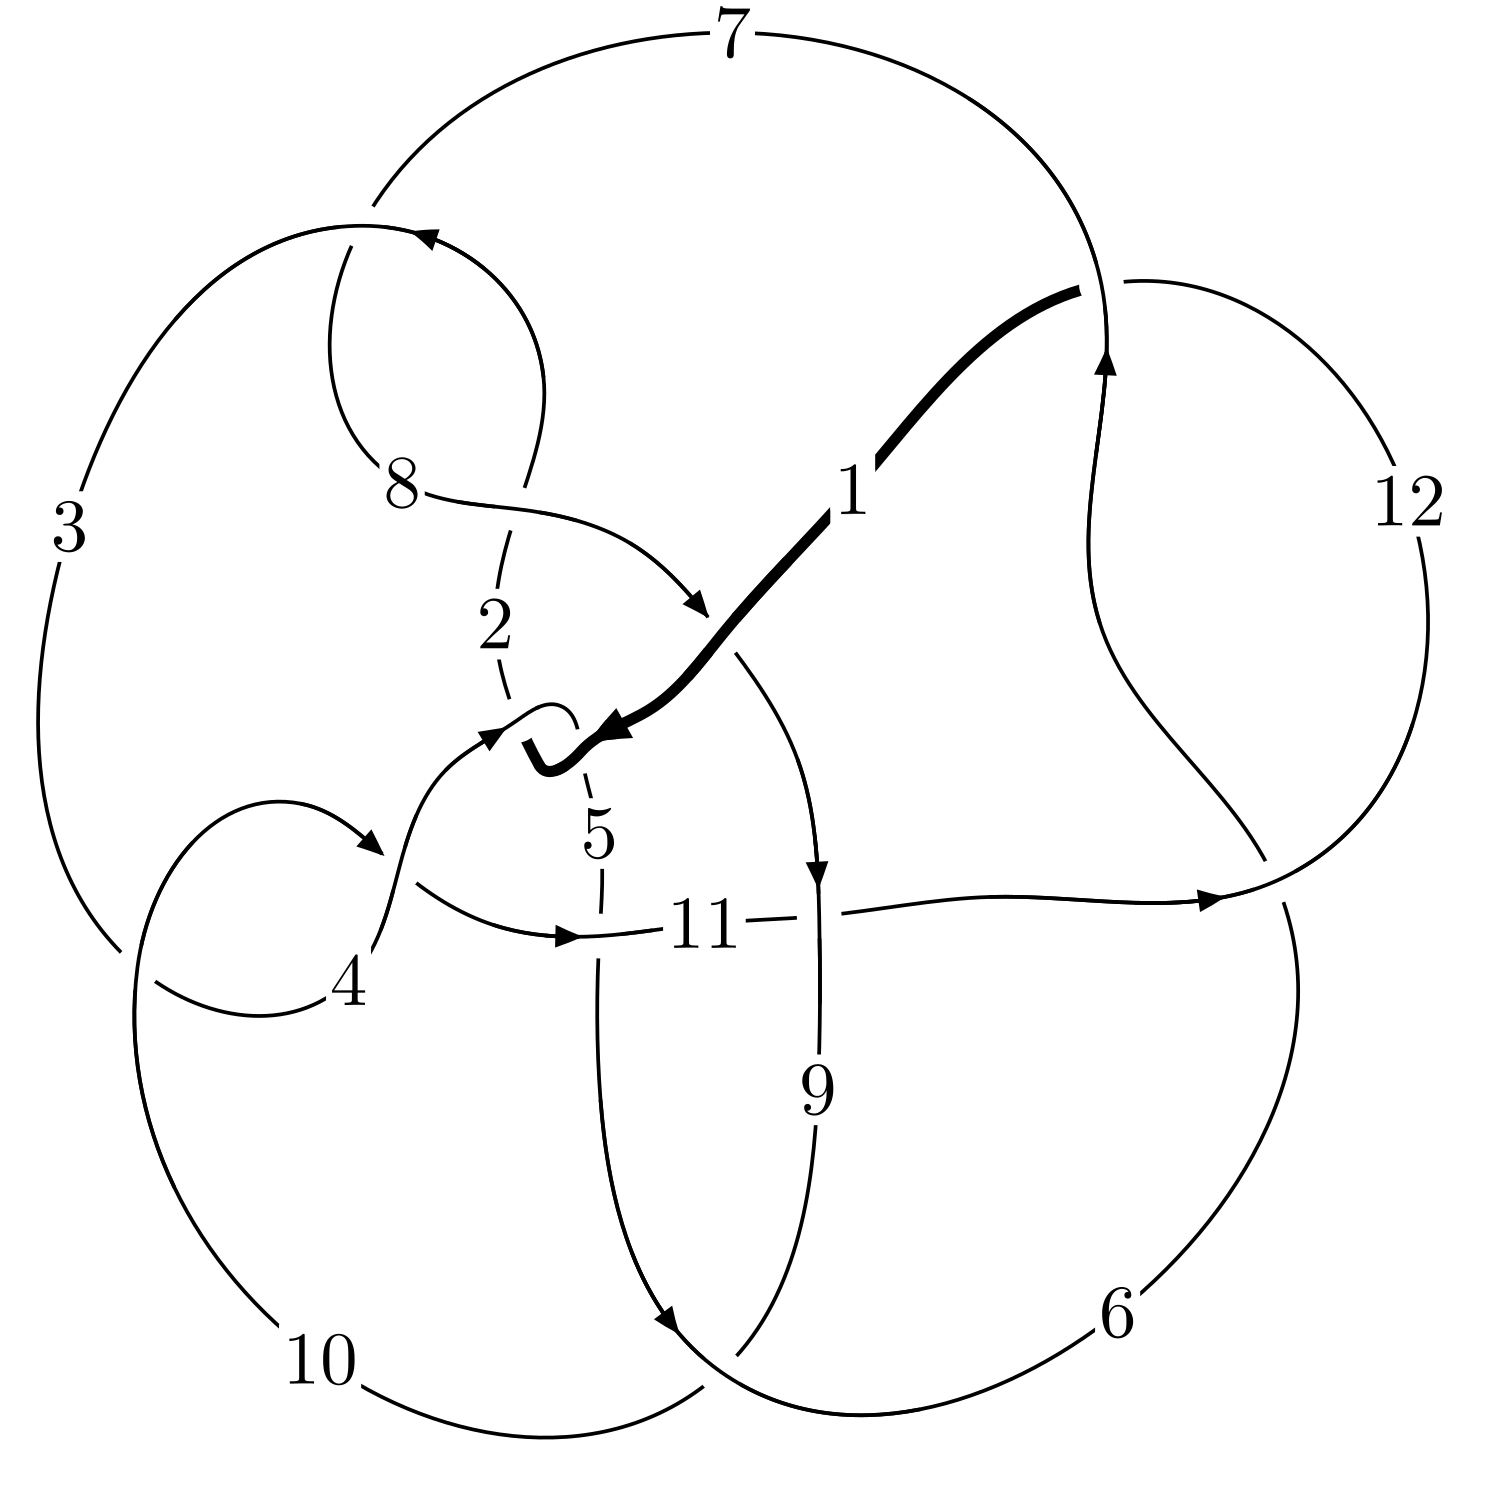
\includegraphics[width=112pt]{../../../GIT/diagram.site/Diagrams/png/2953_12n_0864.png}\\
\ \ \ A knot diagram\footnotemark}&
\allowdisplaybreaks
\textbf{Linearized knot diagam} \\
\cline{2-2}
 &
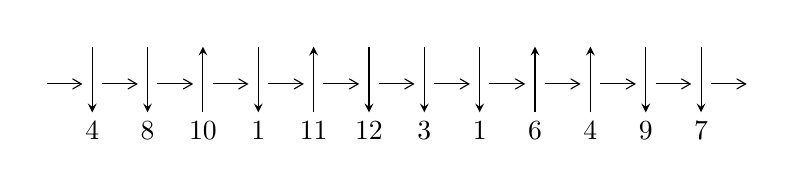
\begin{tikzpicture}[x=20pt, y=17pt]
	% nodes
	\node (C0) at (0, 0) {};
	\node (C1) at (1, 0) {};
	\node (C1U) at (1, +1) {};
	\node (C1D) at (1, -1) {4};

	\node (C2) at (2, 0) {};
	\node (C2U) at (2, +1) {};
	\node (C2D) at (2, -1) {8};

	\node (C3) at (3, 0) {};
	\node (C3U) at (3, +1) {};
	\node (C3D) at (3, -1) {10};

	\node (C4) at (4, 0) {};
	\node (C4U) at (4, +1) {};
	\node (C4D) at (4, -1) {1};

	\node (C5) at (5, 0) {};
	\node (C5U) at (5, +1) {};
	\node (C5D) at (5, -1) {11};

	\node (C6) at (6, 0) {};
	\node (C6U) at (6, +1) {};
	\node (C6D) at (6, -1) {12};

	\node (C7) at (7, 0) {};
	\node (C7U) at (7, +1) {};
	\node (C7D) at (7, -1) {3};

	\node (C8) at (8, 0) {};
	\node (C8U) at (8, +1) {};
	\node (C8D) at (8, -1) {1};

	\node (C9) at (9, 0) {};
	\node (C9U) at (9, +1) {};
	\node (C9D) at (9, -1) {6};

	\node (C10) at (10, 0) {};
	\node (C10U) at (10, +1) {};
	\node (C10D) at (10, -1) {4};

	\node (C11) at (11, 0) {};
	\node (C11U) at (11, +1) {};
	\node (C11D) at (11, -1) {9};

	\node (C12) at (12, 0) {};
	\node (C12U) at (12, +1) {};
	\node (C12D) at (12, -1) {7};
	\node (C13) at (13, 0) {};

	% arrows
	\draw[->,>={angle 60}]
	(C0) edge (C1) (C1) edge (C2) (C2) edge (C3) (C3) edge (C4) (C4) edge (C5) (C5) edge (C6) (C6) edge (C7) (C7) edge (C8) (C8) edge (C9) (C9) edge (C10) (C10) edge (C11) (C11) edge (C12) (C12) edge (C13) ;	\draw[->,>=stealth]
	(C1U) edge (C1D) (C2U) edge (C2D) (C3D) edge (C3U) (C4U) edge (C4D) (C5D) edge (C5U) (C6U) edge (C6D) (C7U) edge (C7D) (C8U) edge (C8D) (C9D) edge (C9U) (C10D) edge (C10U) (C11U) edge (C11D) (C12U) edge (C12D) ;
	\end{tikzpicture} \\
\hhline{~~} \\& 
\textbf{Solving Sequence} \\ \cline{2-2} 
 &
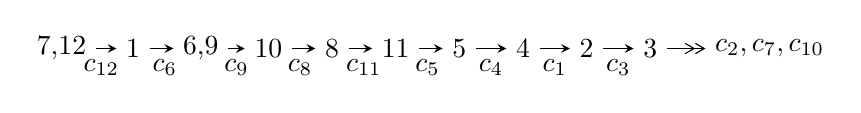
\begin{tikzpicture}[x=23pt, y=7pt]
	% node
	\node (A0) at (-1/8, 0) {7,12};
	\node (A1) at (1, 0) {1};
	\node (A2) at (33/16, 0) {6,9};
	\node (A3) at (25/8, 0) {10};
	\node (A4) at (33/8, 0) {8};
	\node (A5) at (41/8, 0) {11};
	\node (A6) at (49/8, 0) {5};
	\node (A7) at (57/8, 0) {4};
	\node (A8) at (65/8, 0) {2};
	\node (A9) at (73/8, 0) {3};
	\node (C1) at (1/2, -1) {$c_{12}$};
	\node (C2) at (3/2, -1) {$c_{6}$};
	\node (C3) at (21/8, -1) {$c_{9}$};
	\node (C4) at (29/8, -1) {$c_{8}$};
	\node (C5) at (37/8, -1) {$c_{11}$};
	\node (C6) at (45/8, -1) {$c_{5}$};
	\node (C7) at (53/8, -1) {$c_{4}$};
	\node (C8) at (61/8, -1) {$c_{1}$};
	\node (C9) at (69/8, -1) {$c_{3}$};
	\node (A10) at (11, 0) {$c_{2},c_{7},c_{10}$};

	% edge
	\draw[->,>=stealth]	
	(A0) edge (A1) (A1) edge (A2) (A2) edge (A3) (A3) edge (A4) (A4) edge (A5) (A5) edge (A6) (A6) edge (A7) (A7) edge (A8) (A8) edge (A9) ;
	\draw[->>,>={angle 60}]	
	(A9) edge (A10);
\end{tikzpicture} \\ 

\end{tabular} \\

\footnotetext{
The image of knot diagram is generated by the software ``\textbf{Draw programme}" developed by Andrew Bartholomew(\url{http://www.layer8.co.uk/maths/draw/index.htm\#Running-draw}), where we modified some parts for our purpose(\url{https://github.com/CATsTAILs/LinksPainter}).
}\phantom \\ \newline 
\centering \textbf{Ideals for irreducible components\footnotemark of $X_{\text{par}}$} 
 
\begin{align*}
I^u_{1}&=\langle 
1.53286\times10^{291} u^{92}-4.50467\times10^{291} u^{91}+\cdots+3.77692\times10^{291} b+9.71265\times10^{293},\\
\phantom{I^u_{1}}&\phantom{= \langle  }1.02824\times10^{294} u^{92}-2.85879\times10^{294} u^{91}+\cdots+2.69294\times10^{294} a+5.18020\times10^{296},\\
\phantom{I^u_{1}}&\phantom{= \langle  }u^{93}-4 u^{92}+\cdots-4518 u-713\rangle \\
I^u_{2}&=\langle 
2.96874\times10^{21} u^{27}-7.47427\times10^{21} u^{26}+\cdots+2.70703\times10^{22} b-6.60332\times10^{22},\\
\phantom{I^u_{2}}&\phantom{= \langle  }-2.02325\times10^{23} u^{27}+3.57824\times10^{23} u^{26}+\cdots+5.14336\times10^{23} a+2.57084\times10^{24},\\
\phantom{I^u_{2}}&\phantom{= \langle  }u^{28}-3 u^{27}+\cdots-39 u+19\rangle \\
\\
\end{align*}
\raggedright * 2 irreducible components of $\dim_{\mathbb{C}}=0$, with total 121 representations.\\
\footnotetext{All coefficients of polynomials are rational numbers. But the coefficients are sometimes approximated in decimal forms when there is not enough margin.}
\newpage
\renewcommand{\arraystretch}{1}
\centering \section*{I. $I^u_{1}= \langle 1.53\times10^{291} u^{92}-4.50\times10^{291} u^{91}+\cdots+3.78\times10^{291} b+9.71\times10^{293},\;1.03\times10^{294} u^{92}-2.86\times10^{294} u^{91}+\cdots+2.69\times10^{294} a+5.18\times10^{296},\;u^{93}-4 u^{92}+\cdots-4518 u-713 \rangle$}
\flushleft \textbf{(i) Arc colorings}\\
\begin{tabular}{m{7pt} m{180pt} m{7pt} m{180pt} }
\flushright $a_{7}=$&$\begin{pmatrix}0\\u\end{pmatrix}$ \\
\flushright $a_{12}=$&$\begin{pmatrix}1\\0\end{pmatrix}$ \\
\flushright $a_{1}=$&$\begin{pmatrix}1\\u^2\end{pmatrix}$ \\
\flushright $a_{6}=$&$\begin{pmatrix}u\\u\end{pmatrix}$ \\
\flushright $a_{9}=$&$\begin{pmatrix}-0.381829 u^{92}+1.06158 u^{91}+\cdots-1356.84 u-192.362\\-0.405849 u^{92}+1.19268 u^{91}+\cdots-1876.85 u-257.158\end{pmatrix}$ \\
\flushright $a_{10}=$&$\begin{pmatrix}-0.269383 u^{92}+0.806354 u^{91}+\cdots-1215.75 u-167.393\\-0.293403 u^{92}+0.937454 u^{91}+\cdots-1735.76 u-232.189\end{pmatrix}$ \\
\flushright $a_{8}=$&$\begin{pmatrix}-0.198655 u^{92}+0.601956 u^{91}+\cdots-857.280 u-117.454\\-0.0283513 u^{92}+0.170440 u^{91}+\cdots-512.537 u-62.4622\end{pmatrix}$ \\
\flushright $a_{11}=$&$\begin{pmatrix}-0.0836198 u^{92}+0.223873 u^{91}+\cdots-836.341 u-115.884\\0.0332956 u^{92}-0.174545 u^{91}+\cdots-119.532 u-20.4044\end{pmatrix}$ \\
\flushright $a_{5}=$&$\begin{pmatrix}-0.200462 u^{92}+0.633350 u^{91}+\cdots-886.658 u-122.121\\0.179157 u^{92}-0.428392 u^{91}+\cdots+718.139 u+105.165\end{pmatrix}$ \\
\flushright $a_{4}=$&$\begin{pmatrix}0.166083 u^{92}-0.405497 u^{91}+\cdots+735.690 u+103.184\\0.673488 u^{92}-1.84254 u^{91}+\cdots+2910.18 u+409.855\end{pmatrix}$ \\
\flushright $a_{2}=$&$\begin{pmatrix}-0.118324 u^{92}+0.280389 u^{91}+\cdots-580.650 u-81.3422\\-1.46243 u^{92}+4.12770 u^{91}+\cdots-6543.71 u-913.615\end{pmatrix}$ \\
\flushright $a_{3}=$&$\begin{pmatrix}0.153240 u^{92}-0.419507 u^{91}+\cdots+634.309 u+92.1542\\2.16090 u^{92}-6.20878 u^{91}+\cdots+9792.14 u+1358.75\end{pmatrix}$\\&\end{tabular}
\flushleft \textbf{(ii) Obstruction class $= -1$}\\~\\
\flushleft \textbf{(iii) Cusp Shapes $= 1.46340 u^{92}-4.46296 u^{91}+\cdots+8949.13 u+1229.02$}\\~\\
\newpage\renewcommand{\arraystretch}{1}
\flushleft \textbf{(iv) u-Polynomials at the component}\newline \\
\begin{tabular}{m{50pt}|m{274pt}}
Crossings & \hspace{64pt}u-Polynomials at each crossing \\
\hline $$\begin{aligned}c_{1},c_{4}\end{aligned}$$&$\begin{aligned}
&u^{93}-7 u^{92}+\cdots+24150 u-1231
\end{aligned}$\\
\hline $$\begin{aligned}c_{2},c_{7}\end{aligned}$$&$\begin{aligned}
&3(3 u^{93}-7 u^{92}+\cdots+5337 u+845)
\end{aligned}$\\
\hline $$\begin{aligned}c_{3},c_{10}\end{aligned}$$&$\begin{aligned}
&3(3 u^{93}-7 u^{92}+\cdots-29 u-1)
\end{aligned}$\\
\hline $$\begin{aligned}c_{5}\end{aligned}$$&$\begin{aligned}
&u^{93}+u^{92}+\cdots-233909 u+97395
\end{aligned}$\\
\hline $$\begin{aligned}c_{6},c_{12}\end{aligned}$$&$\begin{aligned}
&u^{93}-4 u^{92}+\cdots-4518 u-713
\end{aligned}$\\
\hline $$\begin{aligned}c_{8}\end{aligned}$$&$\begin{aligned}
&u^{93}+5 u^{92}+\cdots-67117955 u+23409813
\end{aligned}$\\
\hline $$\begin{aligned}c_{9}\end{aligned}$$&$\begin{aligned}
&u^{93}+12 u^{91}+\cdots-34564 u-1089
\end{aligned}$\\
\hline $$\begin{aligned}c_{11}\end{aligned}$$&$\begin{aligned}
&9(9 u^{93}-94 u^{92}+\cdots+2774 u-2627)
\end{aligned}$\\
\hline
\end{tabular}\\~\\
\newpage\renewcommand{\arraystretch}{1}
\flushleft \textbf{(v) Riley Polynomials at the component}\newline \\
\begin{tabular}{m{50pt}|m{274pt}}
Crossings & \hspace{64pt}Riley Polynomials at each crossing \\
\hline $$\begin{aligned}c_{1},c_{4}\end{aligned}$$&$\begin{aligned}
&y^{93}-81 y^{92}+\cdots+49128530 y-1515361
\end{aligned}$\\
\hline $$\begin{aligned}c_{2},c_{7}\end{aligned}$$&$\begin{aligned}
&9(9 y^{93}+239 y^{92}+\cdots-1.29958\times10^{7} y-714025)
\end{aligned}$\\
\hline $$\begin{aligned}c_{3},c_{10}\end{aligned}$$&$\begin{aligned}
&9(9 y^{93}-355 y^{92}+\cdots+4293 y-1)
\end{aligned}$\\
\hline $$\begin{aligned}c_{5}\end{aligned}$$&$\begin{aligned}
&y^{93}+35 y^{92}+\cdots-415484901389 y-9485786025
\end{aligned}$\\
\hline $$\begin{aligned}c_{6},c_{12}\end{aligned}$$&$\begin{aligned}
&y^{93}-64 y^{92}+\cdots-3721300 y-508369
\end{aligned}$\\
\hline $$\begin{aligned}c_{8}\end{aligned}$$&$\begin{aligned}
&y^{93}-61 y^{92}+\cdots+33849166602934771 y-548019344694969
\end{aligned}$\\
\hline $$\begin{aligned}c_{9}\end{aligned}$$&$\begin{aligned}
&y^{93}+24 y^{92}+\cdots+318031630 y-1185921
\end{aligned}$\\
\hline $$\begin{aligned}c_{11}\end{aligned}$$&$\begin{aligned}
&81(81 y^{93}-7702 y^{92}+\cdots+2.17902\times10^{8} y-6901129)
\end{aligned}$\\
\hline
\end{tabular}\\~\\
\newpage\flushleft \textbf{(vi) Complex Volumes and Cusp Shapes}
$$\begin{array}{c|c|c}  
\text{Solutions to }I^u_{1}& \I (\text{vol} + \sqrt{-1}CS) & \text{Cusp shape}\\
 \hline 
\begin{aligned}
u &= \phantom{-}0.970806 + 0.203578 I \\
a &= -1.216500 + 0.303430 I \\
b &= -1.087430 - 0.883567 I\end{aligned}
 & -4.33926 - 3.64290 I & \phantom{-0.000000 } 0 \\ \hline\begin{aligned}
u &= \phantom{-}0.970806 - 0.203578 I \\
a &= -1.216500 - 0.303430 I \\
b &= -1.087430 + 0.883567 I\end{aligned}
 & -4.33926 + 3.64290 I & \phantom{-0.000000 } 0 \\ \hline\begin{aligned}
u &= \phantom{-}0.966862 + 0.306426 I \\
a &= \phantom{-}2.12102 - 0.54952 I \\
b &= \phantom{-}1.140770 + 0.801410 I\end{aligned}
 & \phantom{-}4.07438 - 4.79787 I & \phantom{-0.000000 } 0 \\ \hline\begin{aligned}
u &= \phantom{-}0.966862 - 0.306426 I \\
a &= \phantom{-}2.12102 + 0.54952 I \\
b &= \phantom{-}1.140770 - 0.801410 I\end{aligned}
 & \phantom{-}4.07438 + 4.79787 I & \phantom{-0.000000 } 0 \\ \hline\begin{aligned}
u &= -1.01503\phantom{ +0.000000I} \\
a &= \phantom{-}8.34900\phantom{ +0.000000I} \\
b &= \phantom{-}8.17604\phantom{ +0.000000I}\end{aligned}
 & -3.31997\phantom{ +0.000000I} & \phantom{-0.000000 } 0 \\ \hline\begin{aligned}
u &= -1.012850 + 0.093449 I \\
a &= -1.87245 + 0.51826 I \\
b &= -1.030470 - 0.573297 I\end{aligned}
 & -0.912721 + 0.800698 I & \phantom{-0.000000 } 0 \\ \hline\begin{aligned}
u &= -1.012850 - 0.093449 I \\
a &= -1.87245 - 0.51826 I \\
b &= -1.030470 + 0.573297 I\end{aligned}
 & -0.912721 - 0.800698 I & \phantom{-0.000000 } 0 \\ \hline\begin{aligned}
u &= \phantom{-}0.132859 + 1.039890 I \\
a &= \phantom{-}0.073148 + 0.240715 I \\
b &= \phantom{-}0.752841 - 0.369880 I\end{aligned}
 & \phantom{-}2.92510 + 3.79910 I & \phantom{-0.000000 } 0 \\ \hline\begin{aligned}
u &= \phantom{-}0.132859 - 1.039890 I \\
a &= \phantom{-}0.073148 - 0.240715 I \\
b &= \phantom{-}0.752841 + 0.369880 I\end{aligned}
 & \phantom{-}2.92510 - 3.79910 I & \phantom{-0.000000 } 0 \\ \hline\begin{aligned}
u &= \phantom{-}1.072560 + 0.081654 I \\
a &= \phantom{-}1.26700 - 1.92489 I \\
b &= \phantom{-}0.668861 + 0.188400 I\end{aligned}
 & -7.68862 - 0.49446 I & \phantom{-0.000000 } 0\\
 \hline 
 \end{array}$$\newpage$$\begin{array}{c|c|c}  
\text{Solutions to }I^u_{1}& \I (\text{vol} + \sqrt{-1}CS) & \text{Cusp shape}\\
 \hline 
\begin{aligned}
u &= \phantom{-}1.072560 - 0.081654 I \\
a &= \phantom{-}1.26700 + 1.92489 I \\
b &= \phantom{-}0.668861 - 0.188400 I\end{aligned}
 & -7.68862 + 0.49446 I & \phantom{-0.000000 } 0 \\ \hline\begin{aligned}
u &= -0.377912 + 1.043730 I \\
a &= -0.192515 - 0.154482 I \\
b &= -0.966009 + 0.593968 I\end{aligned}
 & -2.83740 - 0.28747 I & \phantom{-0.000000 } 0 \\ \hline\begin{aligned}
u &= -0.377912 - 1.043730 I \\
a &= -0.192515 + 0.154482 I \\
b &= -0.966009 - 0.593968 I\end{aligned}
 & -2.83740 + 0.28747 I & \phantom{-0.000000 } 0 \\ \hline\begin{aligned}
u &= \phantom{-}0.074277 + 0.874223 I \\
a &= -0.175800 + 0.171193 I \\
b &= -1.014600 - 0.732602 I\end{aligned}
 & -3.04223 - 5.10822 I & \phantom{-0.000000 } 0 \\ \hline\begin{aligned}
u &= \phantom{-}0.074277 - 0.874223 I \\
a &= -0.175800 - 0.171193 I \\
b &= -1.014600 + 0.732602 I\end{aligned}
 & -3.04223 + 5.10822 I & \phantom{-0.000000 } 0 \\ \hline\begin{aligned}
u &= -0.090255 + 1.119050 I \\
a &= \phantom{-}0.187340 + 0.249519 I \\
b &= \phantom{-}0.922770 + 0.634829 I\end{aligned}
 & -3.47535 - 4.38011 I & \phantom{-0.000000 } 0 \\ \hline\begin{aligned}
u &= -0.090255 - 1.119050 I \\
a &= \phantom{-}0.187340 - 0.249519 I \\
b &= \phantom{-}0.922770 - 0.634829 I\end{aligned}
 & -3.47535 + 4.38011 I & \phantom{-0.000000 } 0 \\ \hline\begin{aligned}
u &= -1.113330 + 0.179803 I \\
a &= -2.72446 + 1.29296 I \\
b &= -0.580050 + 0.122241 I\end{aligned}
 & -3.79023 + 7.52581 I & \phantom{-0.000000 } 0 \\ \hline\begin{aligned}
u &= -1.113330 - 0.179803 I \\
a &= -2.72446 - 1.29296 I \\
b &= -0.580050 - 0.122241 I\end{aligned}
 & -3.79023 - 7.52581 I & \phantom{-0.000000 } 0 \\ \hline\begin{aligned}
u &= \phantom{-}0.558600 + 0.649221 I \\
a &= -0.330098 - 0.251452 I \\
b &= \phantom{-}0.782526 - 0.802658 I\end{aligned}
 & \phantom{-}5.18841 + 1.02843 I & \phantom{-0.000000 } 0\\
 \hline 
 \end{array}$$\newpage$$\begin{array}{c|c|c}  
\text{Solutions to }I^u_{1}& \I (\text{vol} + \sqrt{-1}CS) & \text{Cusp shape}\\
 \hline 
\begin{aligned}
u &= \phantom{-}0.558600 - 0.649221 I \\
a &= -0.330098 + 0.251452 I \\
b &= \phantom{-}0.782526 + 0.802658 I\end{aligned}
 & \phantom{-}5.18841 - 1.02843 I & \phantom{-0.000000 } 0 \\ \hline\begin{aligned}
u &= -1.155040 + 0.103129 I \\
a &= \phantom{-}1.295920 - 0.012517 I \\
b &= \phantom{-}1.056300 - 0.235080 I\end{aligned}
 & -2.20603 + 0.06003 I & \phantom{-0.000000 } 0 \\ \hline\begin{aligned}
u &= -1.155040 - 0.103129 I \\
a &= \phantom{-}1.295920 + 0.012517 I \\
b &= \phantom{-}1.056300 + 0.235080 I\end{aligned}
 & -2.20603 - 0.06003 I & \phantom{-0.000000 } 0 \\ \hline\begin{aligned}
u &= \phantom{-}1.131360 + 0.303534 I \\
a &= \phantom{-}0.53883 - 1.35038 I \\
b &= \phantom{-}0.74902 - 1.89355 I\end{aligned}
 & -3.07063 - 9.09969 I & \phantom{-0.000000 } 0 \\ \hline\begin{aligned}
u &= \phantom{-}1.131360 - 0.303534 I \\
a &= \phantom{-}0.53883 + 1.35038 I \\
b &= \phantom{-}0.74902 + 1.89355 I\end{aligned}
 & -3.07063 + 9.09969 I & \phantom{-0.000000 } 0 \\ \hline\begin{aligned}
u &= -0.814899 + 0.094544 I \\
a &= -1.27335 + 1.04874 I \\
b &= -0.887354 - 0.420932 I\end{aligned}
 & -0.268157 + 0.195171 I & \phantom{-0.000000 } 0 \\ \hline\begin{aligned}
u &= -0.814899 - 0.094544 I \\
a &= -1.27335 - 1.04874 I \\
b &= -0.887354 + 0.420932 I\end{aligned}
 & -0.268157 - 0.195171 I & \phantom{-0.000000 } 0 \\ \hline\begin{aligned}
u &= \phantom{-}1.185370 + 0.047408 I \\
a &= -1.87899 - 0.66704 I \\
b &= -1.003780 - 0.320920 I\end{aligned}
 & -5.81196 - 2.66335 I & \phantom{-0.000000 } 0 \\ \hline\begin{aligned}
u &= \phantom{-}1.185370 - 0.047408 I \\
a &= -1.87899 + 0.66704 I \\
b &= -1.003780 + 0.320920 I\end{aligned}
 & -5.81196 + 2.66335 I & \phantom{-0.000000 } 0 \\ \hline\begin{aligned}
u &= \phantom{-}0.057798 + 0.804250 I \\
a &= \phantom{-}0.527881 - 0.738120 I \\
b &= \phantom{-}0.332873 + 0.542258 I\end{aligned}
 & \phantom{-}4.07256 + 0.75772 I & \phantom{-}3.56181 + 0. I\phantom{ +0.000000I}\\
 \hline 
 \end{array}$$\newpage$$\begin{array}{c|c|c}  
\text{Solutions to }I^u_{1}& \I (\text{vol} + \sqrt{-1}CS) & \text{Cusp shape}\\
 \hline 
\begin{aligned}
u &= \phantom{-}0.057798 - 0.804250 I \\
a &= \phantom{-}0.527881 + 0.738120 I \\
b &= \phantom{-}0.332873 - 0.542258 I\end{aligned}
 & \phantom{-}4.07256 - 0.75772 I & \phantom{-}3.56181 + 0. I\phantom{ +0.000000I} \\ \hline\begin{aligned}
u &= \phantom{-}1.173730 + 0.250919 I \\
a &= \phantom{-}0.660195 + 0.121675 I \\
b &= \phantom{-}0.551275 - 0.575312 I\end{aligned}
 & \phantom{-}0.34438 - 4.50053 I & \phantom{-0.000000 } 0 \\ \hline\begin{aligned}
u &= \phantom{-}1.173730 - 0.250919 I \\
a &= \phantom{-}0.660195 - 0.121675 I \\
b &= \phantom{-}0.551275 + 0.575312 I\end{aligned}
 & \phantom{-}0.34438 + 4.50053 I & \phantom{-0.000000 } 0 \\ \hline\begin{aligned}
u &= -0.624810 + 1.034520 I \\
a &= \phantom{-}0.155627 - 0.161045 I \\
b &= -0.563147 - 0.194196 I\end{aligned}
 & \phantom{-}1.82620 + 1.45624 I & \phantom{-0.000000 } 0 \\ \hline\begin{aligned}
u &= -0.624810 - 1.034520 I \\
a &= \phantom{-}0.155627 + 0.161045 I \\
b &= -0.563147 + 0.194196 I\end{aligned}
 & \phantom{-}1.82620 - 1.45624 I & \phantom{-0.000000 } 0 \\ \hline\begin{aligned}
u &= \phantom{-}1.214470 + 0.092248 I \\
a &= -1.98528 - 0.50252 I \\
b &= -0.903679 - 0.408944 I\end{aligned}
 & -5.79506 - 2.66432 I & \phantom{-0.000000 } 0 \\ \hline\begin{aligned}
u &= \phantom{-}1.214470 - 0.092248 I \\
a &= -1.98528 + 0.50252 I \\
b &= -0.903679 + 0.408944 I\end{aligned}
 & -5.79506 + 2.66432 I & \phantom{-0.000000 } 0 \\ \hline\begin{aligned}
u &= -1.026460 + 0.671637 I \\
a &= -0.631280 - 0.516781 I \\
b &= -0.823668 + 0.657965 I\end{aligned}
 & \phantom{-}0.27727 + 4.69627 I & \phantom{-0.000000 } 0 \\ \hline\begin{aligned}
u &= -1.026460 - 0.671637 I \\
a &= -0.631280 + 0.516781 I \\
b &= -0.823668 - 0.657965 I\end{aligned}
 & \phantom{-}0.27727 - 4.69627 I & \phantom{-0.000000 } 0 \\ \hline\begin{aligned}
u &= \phantom{-}1.202320 + 0.265022 I \\
a &= -1.266800 + 0.066335 I \\
b &= -1.024440 - 0.779415 I\end{aligned}
 & -4.17035 - 3.28923 I & \phantom{-0.000000 } 0\\
 \hline 
 \end{array}$$\newpage$$\begin{array}{c|c|c}  
\text{Solutions to }I^u_{1}& \I (\text{vol} + \sqrt{-1}CS) & \text{Cusp shape}\\
 \hline 
\begin{aligned}
u &= \phantom{-}1.202320 - 0.265022 I \\
a &= -1.266800 - 0.066335 I \\
b &= -1.024440 + 0.779415 I\end{aligned}
 & -4.17035 + 3.28923 I & \phantom{-0.000000 } 0 \\ \hline\begin{aligned}
u &= \phantom{-}0.428597 + 1.157030 I \\
a &= \phantom{-}0.284631 - 0.357098 I \\
b &= \phantom{-}0.440196 - 0.656343 I\end{aligned}
 & \phantom{-}5.51789 - 0.51100 I & \phantom{-0.000000 } 0 \\ \hline\begin{aligned}
u &= \phantom{-}0.428597 - 1.157030 I \\
a &= \phantom{-}0.284631 + 0.357098 I \\
b &= \phantom{-}0.440196 + 0.656343 I\end{aligned}
 & \phantom{-}5.51789 + 0.51100 I & \phantom{-0.000000 } 0 \\ \hline\begin{aligned}
u &= -0.034127 + 1.237840 I \\
a &= \phantom{-}0.262217 - 0.051286 I \\
b &= \phantom{-}0.974512 - 0.741654 I\end{aligned}
 & -0.91707 + 11.77280 I & \phantom{-0.000000 } 0 \\ \hline\begin{aligned}
u &= -0.034127 - 1.237840 I \\
a &= \phantom{-}0.262217 + 0.051286 I \\
b &= \phantom{-}0.974512 + 0.741654 I\end{aligned}
 & -0.91707 - 11.77280 I & \phantom{-0.000000 } 0 \\ \hline\begin{aligned}
u &= \phantom{-}1.104130 + 0.633695 I \\
a &= \phantom{-}1.61219 - 0.09583 I \\
b &= \phantom{-}1.205820 + 0.638774 I\end{aligned}
 & \phantom{-}3.25583 - 5.58032 I & \phantom{-0.000000 } 0 \\ \hline\begin{aligned}
u &= \phantom{-}1.104130 - 0.633695 I \\
a &= \phantom{-}1.61219 + 0.09583 I \\
b &= \phantom{-}1.205820 - 0.638774 I\end{aligned}
 & \phantom{-}3.25583 + 5.58032 I & \phantom{-0.000000 } 0 \\ \hline\begin{aligned}
u &= -1.259240 + 0.270348 I \\
a &= \phantom{-}1.305300 + 0.136781 I \\
b &= \phantom{-}0.728820 - 1.175300 I\end{aligned}
 & \phantom{-}1.19424 + 6.48567 I & \phantom{-0.000000 } 0 \\ \hline\begin{aligned}
u &= -1.259240 - 0.270348 I \\
a &= \phantom{-}1.305300 - 0.136781 I \\
b &= \phantom{-}0.728820 + 1.175300 I\end{aligned}
 & \phantom{-}1.19424 - 6.48567 I & \phantom{-0.000000 } 0 \\ \hline\begin{aligned}
u &= -1.307360 + 0.038712 I \\
a &= \phantom{-}2.30366 - 0.85775 I \\
b &= \phantom{-}0.678584 - 0.009011 I\end{aligned}
 & -5.16693 - 4.23111 I & \phantom{-0.000000 } 0\\
 \hline 
 \end{array}$$\newpage$$\begin{array}{c|c|c}  
\text{Solutions to }I^u_{1}& \I (\text{vol} + \sqrt{-1}CS) & \text{Cusp shape}\\
 \hline 
\begin{aligned}
u &= -1.307360 - 0.038712 I \\
a &= \phantom{-}2.30366 + 0.85775 I \\
b &= \phantom{-}0.678584 + 0.009011 I\end{aligned}
 & -5.16693 + 4.23111 I & \phantom{-0.000000 } 0 \\ \hline\begin{aligned}
u &= \phantom{-}1.283380 + 0.401547 I \\
a &= \phantom{-}0.795514 - 0.879366 I \\
b &= \phantom{-}0.870337 + 0.078006 I\end{aligned}
 & -8.48265 - 0.61979 I & \phantom{-0.000000 } 0 \\ \hline\begin{aligned}
u &= \phantom{-}1.283380 - 0.401547 I \\
a &= \phantom{-}0.795514 + 0.879366 I \\
b &= \phantom{-}0.870337 - 0.078006 I\end{aligned}
 & -8.48265 + 0.61979 I & \phantom{-0.000000 } 0 \\ \hline\begin{aligned}
u &= \phantom{-}1.284420 + 0.413668 I \\
a &= -0.345035 + 0.490889 I \\
b &= -0.285715 - 0.573754 I\end{aligned}
 & \phantom{-}0.11501 - 5.02565 I & \phantom{-0.000000 } 0 \\ \hline\begin{aligned}
u &= \phantom{-}1.284420 - 0.413668 I \\
a &= -0.345035 - 0.490889 I \\
b &= -0.285715 + 0.573754 I\end{aligned}
 & \phantom{-}0.11501 + 5.02565 I & \phantom{-0.000000 } 0 \\ \hline\begin{aligned}
u &= -1.36052\phantom{ +0.000000I} \\
a &= \phantom{-}1.22117\phantom{ +0.000000I} \\
b &= \phantom{-}1.17430\phantom{ +0.000000I}\end{aligned}
 & -2.32130\phantom{ +0.000000I} & \phantom{-0.000000 } 0 \\ \hline\begin{aligned}
u &= -1.322400 + 0.448761 I \\
a &= -1.81655 - 0.22447 I \\
b &= -1.34813 + 0.89270 I\end{aligned}
 & -7.33144 + 9.91805 I & \phantom{-0.000000 } 0 \\ \hline\begin{aligned}
u &= -1.322400 - 0.448761 I \\
a &= -1.81655 + 0.22447 I \\
b &= -1.34813 - 0.89270 I\end{aligned}
 & -7.33144 - 9.91805 I & \phantom{-0.000000 } 0 \\ \hline\begin{aligned}
u &= -1.358200 + 0.377781 I \\
a &= \phantom{-}1.47648 + 0.38131 I \\
b &= \phantom{-}0.722955 - 0.492677 I\end{aligned}
 & -0.42204 + 3.52052 I & \phantom{-0.000000 } 0 \\ \hline\begin{aligned}
u &= -1.358200 - 0.377781 I \\
a &= \phantom{-}1.47648 - 0.38131 I \\
b &= \phantom{-}0.722955 + 0.492677 I\end{aligned}
 & -0.42204 - 3.52052 I & \phantom{-0.000000 } 0\\
 \hline 
 \end{array}$$\newpage$$\begin{array}{c|c|c}  
\text{Solutions to }I^u_{1}& \I (\text{vol} + \sqrt{-1}CS) & \text{Cusp shape}\\
 \hline 
\begin{aligned}
u &= \phantom{-}1.41210 + 0.09829 I \\
a &= -1.52530 - 0.52170 I \\
b &= -1.38947 - 1.31051 I\end{aligned}
 & -7.64207 - 5.47937 I & \phantom{-0.000000 } 0 \\ \hline\begin{aligned}
u &= \phantom{-}1.41210 - 0.09829 I \\
a &= -1.52530 + 0.52170 I \\
b &= -1.38947 + 1.31051 I\end{aligned}
 & -7.64207 + 5.47937 I & \phantom{-0.000000 } 0 \\ \hline\begin{aligned}
u &= \phantom{-}1.32597 + 0.52524 I \\
a &= \phantom{-}1.332630 - 0.457053 I \\
b &= \phantom{-}1.007260 + 0.638504 I\end{aligned}
 & -0.91883 - 9.40018 I & \phantom{-0.000000 } 0 \\ \hline\begin{aligned}
u &= \phantom{-}1.32597 - 0.52524 I \\
a &= \phantom{-}1.332630 + 0.457053 I \\
b &= \phantom{-}1.007260 - 0.638504 I\end{aligned}
 & -0.91883 + 9.40018 I & \phantom{-0.000000 } 0 \\ \hline\begin{aligned}
u &= \phantom{-}1.24296 + 0.70243 I \\
a &= -0.546032 + 0.779638 I \\
b &= -0.871214 + 0.248362 I\end{aligned}
 & -5.89970 - 0.23874 I & \phantom{-0.000000 } 0 \\ \hline\begin{aligned}
u &= \phantom{-}1.24296 - 0.70243 I \\
a &= -0.546032 - 0.779638 I \\
b &= -0.871214 - 0.248362 I\end{aligned}
 & -5.89970 + 0.23874 I & \phantom{-0.000000 } 0 \\ \hline\begin{aligned}
u &= -0.00838 + 1.43145 I \\
a &= \phantom{-}0.123005 - 0.320045 I \\
b &= -0.237813 - 0.375436 I\end{aligned}
 & \phantom{-}5.10663 - 0.60046 I & \phantom{-0.000000 } 0 \\ \hline\begin{aligned}
u &= -0.00838 - 1.43145 I \\
a &= \phantom{-}0.123005 + 0.320045 I \\
b &= -0.237813 + 0.375436 I\end{aligned}
 & \phantom{-}5.10663 + 0.60046 I & \phantom{-0.000000 } 0 \\ \hline\begin{aligned}
u &= \phantom{-}0.206452 + 0.525183 I \\
a &= \phantom{-}2.42934 - 0.63932 I \\
b &= \phantom{-}0.835132 + 0.833288 I\end{aligned}
 & -0.36815 + 5.85720 I & -1.31662 - 3.27309 I \\ \hline\begin{aligned}
u &= \phantom{-}0.206452 - 0.525183 I \\
a &= \phantom{-}2.42934 + 0.63932 I \\
b &= \phantom{-}0.835132 - 0.833288 I\end{aligned}
 & -0.36815 - 5.85720 I & -1.31662 + 3.27309 I\\
 \hline 
 \end{array}$$\newpage$$\begin{array}{c|c|c}  
\text{Solutions to }I^u_{1}& \I (\text{vol} + \sqrt{-1}CS) & \text{Cusp shape}\\
 \hline 
\begin{aligned}
u &= -1.33863 + 0.54520 I \\
a &= \phantom{-}1.67062 + 0.14858 I \\
b &= \phantom{-}1.39883 - 0.85061 I\end{aligned}
 & -7.46544 + 10.22760 I & \phantom{-0.000000 } 0 \\ \hline\begin{aligned}
u &= -1.33863 - 0.54520 I \\
a &= \phantom{-}1.67062 - 0.14858 I \\
b &= \phantom{-}1.39883 + 0.85061 I\end{aligned}
 & -7.46544 - 10.22760 I & \phantom{-0.000000 } 0 \\ \hline\begin{aligned}
u &= \phantom{-}1.42171 + 0.34511 I \\
a &= -1.65249 - 0.02833 I \\
b &= -1.39250 - 0.99250 I\end{aligned}
 & -8.59422 - 4.37880 I & \phantom{-0.000000 } 0 \\ \hline\begin{aligned}
u &= \phantom{-}1.42171 - 0.34511 I \\
a &= -1.65249 + 0.02833 I \\
b &= -1.39250 + 0.99250 I\end{aligned}
 & -8.59422 + 4.37880 I & \phantom{-0.000000 } 0 \\ \hline\begin{aligned}
u &= -0.490424 + 0.192252 I \\
a &= \phantom{-}2.02573 - 1.32129 I \\
b &= \phantom{-}0.775835 - 0.910483 I\end{aligned}
 & -2.77711 + 0.92123 I & -2.40188 - 0.43411 I \\ \hline\begin{aligned}
u &= -0.490424 - 0.192252 I \\
a &= \phantom{-}2.02573 + 1.32129 I \\
b &= \phantom{-}0.775835 + 0.910483 I\end{aligned}
 & -2.77711 - 0.92123 I & -2.40188 + 0.43411 I \\ \hline\begin{aligned}
u &= \phantom{-}1.41052 + 0.56464 I \\
a &= \phantom{-}1.63990 - 0.17204 I \\
b &= \phantom{-}1.32824 + 0.93343 I\end{aligned}
 & -5.4749 - 18.0350 I & \phantom{-0.000000 } 0 \\ \hline\begin{aligned}
u &= \phantom{-}1.41052 - 0.56464 I \\
a &= \phantom{-}1.63990 + 0.17204 I \\
b &= \phantom{-}1.32824 - 0.93343 I\end{aligned}
 & -5.4749 + 18.0350 I & \phantom{-0.000000 } 0 \\ \hline\begin{aligned}
u &= -0.373413 + 0.292324 I \\
a &= -1.23651 + 2.18723 I \\
b &= -0.681200 - 0.818287 I\end{aligned}
 & -1.66413 - 5.49946 I & -1.46246 + 5.05508 I \\ \hline\begin{aligned}
u &= -0.373413 - 0.292324 I \\
a &= -1.23651 - 2.18723 I \\
b &= -0.681200 + 0.818287 I\end{aligned}
 & -1.66413 + 5.49946 I & -1.46246 - 5.05508 I\\
 \hline 
 \end{array}$$\newpage$$\begin{array}{c|c|c}  
\text{Solutions to }I^u_{1}& \I (\text{vol} + \sqrt{-1}CS) & \text{Cusp shape}\\
 \hline 
\begin{aligned}
u &= -1.34540 + 0.73623 I \\
a &= -0.598439 - 0.635209 I \\
b &= -0.986576 + 0.010327 I\end{aligned}
 & -5.63674 + 7.02123 I & \phantom{-0.000000 } 0 \\ \hline\begin{aligned}
u &= -1.34540 - 0.73623 I \\
a &= -0.598439 + 0.635209 I \\
b &= -0.986576 - 0.010327 I\end{aligned}
 & -5.63674 - 7.02123 I & \phantom{-0.000000 } 0 \\ \hline\begin{aligned}
u &= -1.43121 + 0.61007 I \\
a &= -1.009230 + 0.287321 I \\
b &= -0.948448 + 0.982762 I\end{aligned}
 & \phantom{-}0.35724 + 7.41586 I & \phantom{-0.000000 } 0 \\ \hline\begin{aligned}
u &= -1.43121 - 0.61007 I \\
a &= -1.009230 - 0.287321 I \\
b &= -0.948448 - 0.982762 I\end{aligned}
 & \phantom{-}0.35724 - 7.41586 I & \phantom{-0.000000 } 0 \\ \hline\begin{aligned}
u &= -0.077867 + 0.405146 I \\
a &= -2.14768 - 1.36570 I \\
b &= \phantom{-}0.551812 + 0.744999 I\end{aligned}
 & \phantom{-}4.92357 - 3.65063 I & \phantom{-}1.05797 + 12.64547 I \\ \hline\begin{aligned}
u &= -0.077867 - 0.405146 I \\
a &= -2.14768 + 1.36570 I \\
b &= \phantom{-}0.551812 - 0.744999 I\end{aligned}
 & \phantom{-}4.92357 + 3.65063 I & \phantom{-}1.05797 - 12.64547 I \\ \hline\begin{aligned}
u &= -0.181026 + 0.342017 I \\
a &= \phantom{-}0.500745 - 0.770110 I \\
b &= -0.426902 + 0.358041 I\end{aligned}
 & -0.200991 + 0.958280 I & -3.95907 - 6.99416 I \\ \hline\begin{aligned}
u &= -0.181026 - 0.342017 I \\
a &= \phantom{-}0.500745 + 0.770110 I \\
b &= -0.426902 - 0.358041 I\end{aligned}
 & -0.200991 - 0.958280 I & -3.95907 + 6.99416 I \\ \hline\begin{aligned}
u &= -0.137092 + 0.322899 I \\
a &= -2.24872 - 0.63912 I \\
b &= -0.744226 + 1.001560 I\end{aligned}
 & -1.96423 + 1.03167 I & \phantom{-}0.423681 + 0.449105 I \\ \hline\begin{aligned}
u &= -0.137092 - 0.322899 I \\
a &= -2.24872 + 0.63912 I \\
b &= -0.744226 - 1.001560 I\end{aligned}
 & -1.96423 - 1.03167 I & \phantom{-}0.423681 - 0.449105 I\\
 \hline 
 \end{array}$$\newpage$$\begin{array}{c|c|c}  
\text{Solutions to }I^u_{1}& \I (\text{vol} + \sqrt{-1}CS) & \text{Cusp shape}\\
 \hline 
\begin{aligned}
u &= \phantom{-}1.69081\phantom{ +0.000000I} \\
a &= \phantom{-}1.34078\phantom{ +0.000000I} \\
b &= \phantom{-}0.835244\phantom{ +0.000000I}\end{aligned}
 & -10.1731\phantom{ +0.000000I} & \phantom{-0.000000 } 0 \\ \hline\begin{aligned}
u &= -1.63854 + 0.53885 I \\
a &= \phantom{-}0.671092 + 0.461091 I \\
b &= \phantom{-}0.850672 + 0.119820 I\end{aligned}
 & -5.87559 - 4.83598 I & \phantom{-0.000000 } 0 \\ \hline\begin{aligned}
u &= -1.63854 - 0.53885 I \\
a &= \phantom{-}0.671092 - 0.461091 I \\
b &= \phantom{-}0.850672 - 0.119820 I\end{aligned}
 & -5.87559 + 4.83598 I & \phantom{-0.000000 } 0\\
 \hline 
 \end{array}$$\newpage\newpage\renewcommand{\arraystretch}{1}
\centering \section*{II. $I^u_{2}= \langle 2.97\times10^{21} u^{27}-7.47\times10^{21} u^{26}+\cdots+2.71\times10^{22} b-6.60\times10^{22},\;-2.02\times10^{23} u^{27}+3.58\times10^{23} u^{26}+\cdots+5.14\times10^{23} a+2.57\times10^{24},\;u^{28}-3 u^{27}+\cdots-39 u+19 \rangle$}
\flushleft \textbf{(i) Arc colorings}\\
\begin{tabular}{m{7pt} m{180pt} m{7pt} m{180pt} }
\flushright $a_{7}=$&$\begin{pmatrix}0\\u\end{pmatrix}$ \\
\flushright $a_{12}=$&$\begin{pmatrix}1\\0\end{pmatrix}$ \\
\flushright $a_{1}=$&$\begin{pmatrix}1\\u^2\end{pmatrix}$ \\
\flushright $a_{6}=$&$\begin{pmatrix}u\\u\end{pmatrix}$ \\
\flushright $a_{9}=$&$\begin{pmatrix}0.393370 u^{27}-0.695700 u^{26}+\cdots+7.51834 u-4.99835\\-0.109668 u^{27}+0.276105 u^{26}+\cdots-1.97895 u+2.43932\end{pmatrix}$ \\
\flushright $a_{10}=$&$\begin{pmatrix}-0.146103 u^{27}+0.419124 u^{26}+\cdots-3.87896 u+5.21050\\-0.649141 u^{27}+1.39093 u^{26}+\cdots-13.3763 u+12.6482\end{pmatrix}$ \\
\flushright $a_{8}=$&$\begin{pmatrix}-0.348178 u^{27}+0.716088 u^{26}+\cdots-5.87861 u+6.64478\\-0.972474 u^{27}+1.99708 u^{26}+\cdots-19.5910 u+17.8836\end{pmatrix}$ \\
\flushright $a_{11}=$&$\begin{pmatrix}0.312529 u^{27}-0.559950 u^{26}+\cdots+8.78283 u-4.64925\\0.185894 u^{27}-0.266959 u^{26}+\cdots+6.09066 u-3.17580\end{pmatrix}$ \\
\flushright $a_{5}=$&$\begin{pmatrix}-0.435301 u^{27}+0.840298 u^{26}+\cdots-8.78720 u+7.15731\\-0.502956 u^{27}+0.904377 u^{26}+\cdots-8.48786 u+8.02330\end{pmatrix}$ \\
\flushright $a_{4}=$&$\begin{pmatrix}-0.318183 u^{27}+0.702283 u^{26}+\cdots-7.38719 u+6.33412\\-0.165206 u^{27}+0.439800 u^{26}+\cdots-2.39284 u+3.96984\end{pmatrix}$ \\
\flushright $a_{2}=$&$\begin{pmatrix}-0.100290 u^{27}+0.134408 u^{26}+\cdots-4.69317 u-0.385276\\-0.263668 u^{27}+0.256350 u^{26}+\cdots-2.86034 u+0.586162\end{pmatrix}$ \\
\flushright $a_{3}=$&$\begin{pmatrix}0.361386 u^{27}-0.629649 u^{26}+\cdots+5.94865 u-5.75225\\0.812419 u^{27}-1.34489 u^{26}+\cdots+16.6198 u-11.1591\end{pmatrix}$\\&\end{tabular}
\flushleft \textbf{(ii) Obstruction class $= 1$}\\~\\
\flushleft \textbf{(iii) Cusp Shapes $= \frac{36346825326951087058817}{730899156647188975048731} u^{27}-\frac{381420569456833601389550}{730899156647188975048731} u^{26}+\cdots+\frac{3998852031337486870792207}{730899156647188975048731} u-\frac{9592325382796608124681696}{730899156647188975048731}$}\\~\\
\newpage\renewcommand{\arraystretch}{1}
\flushleft \textbf{(iv) u-Polynomials at the component}\newline \\
\begin{tabular}{m{50pt}|m{274pt}}
Crossings & \hspace{64pt}u-Polynomials at each crossing \\
\hline $$\begin{aligned}c_{1}\end{aligned}$$&$\begin{aligned}
&u^{28}-4 u^{27}+\cdots+3 u+1
\end{aligned}$\\
\hline $$\begin{aligned}c_{2}\end{aligned}$$&$\begin{aligned}
&3(3 u^{28}-4 u^{27}+\cdots-2 u-1)
\end{aligned}$\\
\hline $$\begin{aligned}c_{3}\end{aligned}$$&$\begin{aligned}
&3(3 u^{28}-4 u^{27}+\cdots-4 u-1)
\end{aligned}$\\
\hline $$\begin{aligned}c_{4}\end{aligned}$$&$\begin{aligned}
&u^{28}+4 u^{27}+\cdots-3 u+1
\end{aligned}$\\
\hline $$\begin{aligned}c_{5}\end{aligned}$$&$\begin{aligned}
&u^{28}+4 u^{26}+\cdots+20 u+183
\end{aligned}$\\
\hline $$\begin{aligned}c_{6}\end{aligned}$$&$\begin{aligned}
&u^{28}+3 u^{27}+\cdots+39 u+19
\end{aligned}$\\
\hline $$\begin{aligned}c_{7}\end{aligned}$$&$\begin{aligned}
&3(3 u^{28}+4 u^{27}+\cdots+2 u-1)
\end{aligned}$\\
\hline $$\begin{aligned}c_{8}\end{aligned}$$&$\begin{aligned}
&u^{28}+4 u^{27}+\cdots-550 u-393
\end{aligned}$\\
\hline $$\begin{aligned}c_{9}\end{aligned}$$&$\begin{aligned}
&u^{28}+u^{27}+\cdots-91 u-9
\end{aligned}$\\
\hline $$\begin{aligned}c_{10}\end{aligned}$$&$\begin{aligned}
&3(3 u^{28}+4 u^{27}+\cdots+4 u-1)
\end{aligned}$\\
\hline $$\begin{aligned}c_{11}\end{aligned}$$&$\begin{aligned}
&9(9 u^{28}+11 u^{27}+\cdots-9 u-1)
\end{aligned}$\\
\hline $$\begin{aligned}c_{12}\end{aligned}$$&$\begin{aligned}
&u^{28}-3 u^{27}+\cdots-39 u+19
\end{aligned}$\\
\hline
\end{tabular}\\~\\
\newpage\renewcommand{\arraystretch}{1}
\flushleft \textbf{(v) Riley Polynomials at the component}\newline \\
\begin{tabular}{m{50pt}|m{274pt}}
Crossings & \hspace{64pt}Riley Polynomials at each crossing \\
\hline $$\begin{aligned}c_{1},c_{4}\end{aligned}$$&$\begin{aligned}
&y^{28}-20 y^{27}+\cdots+19 y+1
\end{aligned}$\\
\hline $$\begin{aligned}c_{2},c_{7}\end{aligned}$$&$\begin{aligned}
&9(9 y^{28}+128 y^{27}+\cdots+16 y+1)
\end{aligned}$\\
\hline $$\begin{aligned}c_{3},c_{10}\end{aligned}$$&$\begin{aligned}
&9(9 y^{28}-142 y^{27}+\cdots-20 y+1)
\end{aligned}$\\
\hline $$\begin{aligned}c_{5}\end{aligned}$$&$\begin{aligned}
&y^{28}+8 y^{27}+\cdots+73898 y+33489
\end{aligned}$\\
\hline $$\begin{aligned}c_{6},c_{12}\end{aligned}$$&$\begin{aligned}
&y^{28}-19 y^{27}+\cdots+1557 y+361
\end{aligned}$\\
\hline $$\begin{aligned}c_{8}\end{aligned}$$&$\begin{aligned}
&y^{28}-20 y^{27}+\cdots-1881574 y+154449
\end{aligned}$\\
\hline $$\begin{aligned}c_{9}\end{aligned}$$&$\begin{aligned}
&y^{28}+9 y^{27}+\cdots-8281 y+81
\end{aligned}$\\
\hline $$\begin{aligned}c_{11}\end{aligned}$$&$\begin{aligned}
&81(81 y^{28}-769 y^{27}+\cdots-17 y+1)
\end{aligned}$\\
\hline
\end{tabular}\\~\\
\newpage\flushleft \textbf{(vi) Complex Volumes and Cusp Shapes}
$$\begin{array}{c|c|c}  
\text{Solutions to }I^u_{2}& \I (\text{vol} + \sqrt{-1}CS) & \text{Cusp shape}\\
 \hline 
\begin{aligned}
u &= \phantom{-}0.521754 + 0.880090 I \\
a &= \phantom{-}0.382943 - 0.169516 I \\
b &= -0.411507 + 0.021686 I\end{aligned}
 & \phantom{-}2.01994 - 1.83061 I & \phantom{-}1.50906 + 8.83594 I \\ \hline\begin{aligned}
u &= \phantom{-}0.521754 - 0.880090 I \\
a &= \phantom{-}0.382943 + 0.169516 I \\
b &= -0.411507 - 0.021686 I\end{aligned}
 & \phantom{-}2.01994 + 1.83061 I & \phantom{-}1.50906 - 8.83594 I \\ \hline\begin{aligned}
u &= \phantom{-}1.004320 + 0.286358 I \\
a &= \phantom{-}1.207610 + 0.017108 I \\
b &= -0.009872 - 0.775666 I\end{aligned}
 & -2.87333 - 7.20168 I & -3.49158 + 5.74174 I \\ \hline\begin{aligned}
u &= \phantom{-}1.004320 - 0.286358 I \\
a &= \phantom{-}1.207610 - 0.017108 I \\
b &= -0.009872 + 0.775666 I\end{aligned}
 & -2.87333 + 7.20168 I & -3.49158 - 5.74174 I \\ \hline\begin{aligned}
u &= -1.070500 + 0.186519 I \\
a &= \phantom{-}0.88674 + 1.77203 I \\
b &= \phantom{-}0.680259 - 0.192286 I\end{aligned}
 & -7.57229 + 0.82853 I & -2.46578 - 12.32293 I \\ \hline\begin{aligned}
u &= -1.070500 - 0.186519 I \\
a &= \phantom{-}0.88674 - 1.77203 I \\
b &= \phantom{-}0.680259 + 0.192286 I\end{aligned}
 & -7.57229 - 0.82853 I & -2.46578 + 12.32293 I \\ \hline\begin{aligned}
u &= \phantom{-}0.562054 + 0.961301 I \\
a &= \phantom{-}0.029738 - 0.391667 I \\
b &= \phantom{-}0.648409 - 0.815439 I\end{aligned}
 & \phantom{-}6.74803 + 0.55431 I & \phantom{-}4.39621 - 1.64176 I \\ \hline\begin{aligned}
u &= \phantom{-}0.562054 - 0.961301 I \\
a &= \phantom{-}0.029738 + 0.391667 I \\
b &= \phantom{-}0.648409 + 0.815439 I\end{aligned}
 & \phantom{-}6.74803 - 0.55431 I & \phantom{-}4.39621 + 1.64176 I \\ \hline\begin{aligned}
u &= -1.12047\phantom{ +0.000000I} \\
a &= \phantom{-}2.69049\phantom{ +0.000000I} \\
b &= \phantom{-}2.60517\phantom{ +0.000000I}\end{aligned}
 & -3.44038\phantom{ +0.000000I} & -18.1190\phantom{ +0.000000I} \\ \hline\begin{aligned}
u &= \phantom{-}1.048530 + 0.497158 I \\
a &= \phantom{-}1.81281 - 0.12113 I \\
b &= \phantom{-}1.14446 + 0.91674 I\end{aligned}
 & \phantom{-}5.07440 - 5.77041 I & \phantom{-}2.11038 + 6.19669 I\\
 \hline 
 \end{array}$$\newpage$$\begin{array}{c|c|c}  
\text{Solutions to }I^u_{2}& \I (\text{vol} + \sqrt{-1}CS) & \text{Cusp shape}\\
 \hline 
\begin{aligned}
u &= \phantom{-}1.048530 - 0.497158 I \\
a &= \phantom{-}1.81281 + 0.12113 I \\
b &= \phantom{-}1.14446 - 0.91674 I\end{aligned}
 & \phantom{-}5.07440 + 5.77041 I & \phantom{-}2.11038 - 6.19669 I \\ \hline\begin{aligned}
u &= -1.255070 + 0.285789 I \\
a &= \phantom{-}1.296300 + 0.417482 I \\
b &= \phantom{-}0.676477 - 0.994621 I\end{aligned}
 & \phantom{-}1.63709 + 6.17925 I & \phantom{-}3.37825 - 3.29613 I \\ \hline\begin{aligned}
u &= -1.255070 - 0.285789 I \\
a &= \phantom{-}1.296300 - 0.417482 I \\
b &= \phantom{-}0.676477 + 0.994621 I\end{aligned}
 & \phantom{-}1.63709 - 6.17925 I & \phantom{-}3.37825 + 3.29613 I \\ \hline\begin{aligned}
u &= \phantom{-}1.340010 + 0.147694 I \\
a &= -1.43207 + 0.40771 I \\
b &= -0.460042 + 0.447927 I\end{aligned}
 & -4.26015 + 4.72994 I & -3.25602 - 6.00078 I \\ \hline\begin{aligned}
u &= \phantom{-}1.340010 - 0.147694 I \\
a &= -1.43207 - 0.40771 I \\
b &= -0.460042 - 0.447927 I\end{aligned}
 & -4.26015 - 4.72994 I & -3.25602 + 6.00078 I \\ \hline\begin{aligned}
u &= \phantom{-}1.283280 + 0.418019 I \\
a &= -1.129020 + 0.697209 I \\
b &= -0.681608 - 0.385401 I\end{aligned}
 & -0.85125 - 2.97639 I & -7.07571 - 0.53480 I \\ \hline\begin{aligned}
u &= \phantom{-}1.283280 - 0.418019 I \\
a &= -1.129020 - 0.697209 I \\
b &= -0.681608 + 0.385401 I\end{aligned}
 & -0.85125 + 2.97639 I & -7.07571 + 0.53480 I \\ \hline\begin{aligned}
u &= \phantom{-}1.396940 + 0.174140 I \\
a &= -1.63173 - 0.37311 I \\
b &= -1.43554 - 1.19718 I\end{aligned}
 & -7.54617 - 5.02484 I & -4.07792 - 1.75277 I \\ \hline\begin{aligned}
u &= \phantom{-}1.396940 - 0.174140 I \\
a &= -1.63173 + 0.37311 I \\
b &= -1.43554 + 1.19718 I\end{aligned}
 & -7.54617 + 5.02484 I & -4.07792 + 1.75277 I \\ \hline\begin{aligned}
u &= -0.294127 + 0.476992 I \\
a &= -1.81518 - 0.27843 I \\
b &= \phantom{-}0.543604 + 0.583954 I\end{aligned}
 & \phantom{-}4.95221 - 3.15515 I & \phantom{-}2.16472 - 2.64497 I\\
 \hline 
 \end{array}$$\newpage$$\begin{array}{c|c|c}  
\text{Solutions to }I^u_{2}& \I (\text{vol} + \sqrt{-1}CS) & \text{Cusp shape}\\
 \hline 
\begin{aligned}
u &= -0.294127 - 0.476992 I \\
a &= -1.81518 + 0.27843 I \\
b &= \phantom{-}0.543604 - 0.583954 I\end{aligned}
 & \phantom{-}4.95221 + 3.15515 I & \phantom{-}2.16472 + 2.64497 I \\ \hline\begin{aligned}
u &= \phantom{-}0.057545 + 0.467455 I \\
a &= \phantom{-}0.646815 + 0.815476 I \\
b &= -0.894668 + 0.734654 I\end{aligned}
 & -2.82369 + 2.83577 I & -2.08018 - 2.99142 I \\ \hline\begin{aligned}
u &= \phantom{-}0.057545 - 0.467455 I \\
a &= \phantom{-}0.646815 - 0.815476 I \\
b &= -0.894668 - 0.734654 I\end{aligned}
 & -2.82369 - 2.83577 I & -2.08018 + 2.99142 I \\ \hline\begin{aligned}
u &= -0.26281 + 1.52272 I \\
a &= -0.052675 - 0.290436 I \\
b &= -0.419220 - 0.307941 I\end{aligned}
 & \phantom{-}4.95254 + 0.16143 I & -7.70420 + 4.24851 I \\ \hline\begin{aligned}
u &= -0.26281 - 1.52272 I \\
a &= -0.052675 + 0.290436 I \\
b &= -0.419220 + 0.307941 I\end{aligned}
 & \phantom{-}4.95254 - 0.16143 I & -7.70420 - 4.24851 I \\ \hline\begin{aligned}
u &= -1.41891 + 0.65551 I \\
a &= -0.943900 + 0.122189 I \\
b &= -0.887039 + 0.838068 I\end{aligned}
 & \phantom{-}0.74318 + 7.19731 I & \phantom{-}4.06191 - 4.63819 I \\ \hline\begin{aligned}
u &= -1.41891 - 0.65551 I \\
a &= -0.943900 - 0.122189 I \\
b &= -0.887039 - 0.838068 I\end{aligned}
 & \phantom{-}0.74318 - 7.19731 I & \phantom{-}4.06191 + 4.63819 I \\ \hline\begin{aligned}
u &= -1.70552\phantom{ +0.000000I} \\
a &= -1.32420\phantom{ +0.000000I} \\
b &= -0.814815\phantom{ +0.000000I}\end{aligned}
 & -10.1201\phantom{ +0.000000I} & \phantom{-}71.7450\phantom{ +0.000000I}\\
 \hline 
 \end{array}$$\newpage
\newpage\renewcommand{\arraystretch}{1}
\centering \section*{ III. u-Polynomials}
\begin{tabular}{m{50pt}|m{274pt}}
Crossings & \hspace{64pt}u-Polynomials at each crossing \\
\hline $$\begin{aligned}c_{1}\end{aligned}$$&$\begin{aligned}
&(u^{28}-4 u^{27}+\cdots+3 u+1)(u^{93}-7 u^{92}+\cdots+24150 u-1231)
\end{aligned}$\\
\hline $$\begin{aligned}c_{2}\end{aligned}$$&$\begin{aligned}
&9(3 u^{28}-4 u^{27}+\cdots-2 u-1)(3 u^{93}-7 u^{92}+\cdots+5337 u+845)
\end{aligned}$\\
\hline $$\begin{aligned}c_{3}\end{aligned}$$&$\begin{aligned}
&9(3 u^{28}-4 u^{27}+\cdots-4 u-1)(3 u^{93}-7 u^{92}+\cdots-29 u-1)
\end{aligned}$\\
\hline $$\begin{aligned}c_{4}\end{aligned}$$&$\begin{aligned}
&(u^{28}+4 u^{27}+\cdots-3 u+1)(u^{93}-7 u^{92}+\cdots+24150 u-1231)
\end{aligned}$\\
\hline $$\begin{aligned}c_{5}\end{aligned}$$&$\begin{aligned}
&(u^{28}+4 u^{26}+\cdots+20 u+183)(u^{93}+u^{92}+\cdots-233909 u+97395)
\end{aligned}$\\
\hline $$\begin{aligned}c_{6}\end{aligned}$$&$\begin{aligned}
&(u^{28}+3 u^{27}+\cdots+39 u+19)(u^{93}-4 u^{92}+\cdots-4518 u-713)
\end{aligned}$\\
\hline $$\begin{aligned}c_{7}\end{aligned}$$&$\begin{aligned}
&9(3 u^{28}+4 u^{27}+\cdots+2 u-1)(3 u^{93}-7 u^{92}+\cdots+5337 u+845)
\end{aligned}$\\
\hline $$\begin{aligned}c_{8}\end{aligned}$$&$\begin{aligned}
&(u^{28}+4 u^{27}+\cdots-550 u-393)\\
&\cdot(u^{93}+5 u^{92}+\cdots-67117955 u+23409813)
\end{aligned}$\\
\hline $$\begin{aligned}c_{9}\end{aligned}$$&$\begin{aligned}
&(u^{28}+u^{27}+\cdots-91 u-9)(u^{93}+12 u^{91}+\cdots-34564 u-1089)
\end{aligned}$\\
\hline $$\begin{aligned}c_{10}\end{aligned}$$&$\begin{aligned}
&9(3 u^{28}+4 u^{27}+\cdots+4 u-1)(3 u^{93}-7 u^{92}+\cdots-29 u-1)
\end{aligned}$\\
\hline $$\begin{aligned}c_{11}\end{aligned}$$&$\begin{aligned}
&81(9 u^{28}+11 u^{27}+\cdots-9 u-1)(9 u^{93}-94 u^{92}+\cdots+2774 u-2627)
\end{aligned}$\\
\hline $$\begin{aligned}c_{12}\end{aligned}$$&$\begin{aligned}
&(u^{28}-3 u^{27}+\cdots-39 u+19)(u^{93}-4 u^{92}+\cdots-4518 u-713)
\end{aligned}$\\
\hline
\end{tabular}\newpage\renewcommand{\arraystretch}{1}
\centering \section*{ IV. Riley Polynomials}
\begin{tabular}{m{50pt}|m{274pt}}
Crossings & \hspace{64pt}Riley Polynomials at each crossing \\
\hline $$\begin{aligned}c_{1},c_{4}\end{aligned}$$&$\begin{aligned}
&(y^{28}-20 y^{27}+\cdots+19 y+1)\\
&\cdot(y^{93}-81 y^{92}+\cdots+49128530 y-1515361)
\end{aligned}$\\
\hline $$\begin{aligned}c_{2},c_{7}\end{aligned}$$&$\begin{aligned}
&81(9 y^{28}+128 y^{27}+\cdots+16 y+1)\\
&\cdot(9 y^{93}+239 y^{92}+\cdots-12995791 y-714025)
\end{aligned}$\\
\hline $$\begin{aligned}c_{3},c_{10}\end{aligned}$$&$\begin{aligned}
&81(9 y^{28}-142 y^{27}+\cdots-20 y+1)(9 y^{93}-355 y^{92}+\cdots+4293 y-1)
\end{aligned}$\\
\hline $$\begin{aligned}c_{5}\end{aligned}$$&$\begin{aligned}
&(y^{28}+8 y^{27}+\cdots+73898 y+33489)\\
&\cdot(y^{93}+35 y^{92}+\cdots-415484901389 y-9485786025)
\end{aligned}$\\
\hline $$\begin{aligned}c_{6},c_{12}\end{aligned}$$&$\begin{aligned}
&(y^{28}-19 y^{27}+\cdots+1557 y+361)\\
&\cdot(y^{93}-64 y^{92}+\cdots-3721300 y-508369)
\end{aligned}$\\
\hline $$\begin{aligned}c_{8}\end{aligned}$$&$\begin{aligned}
&(y^{28}-20 y^{27}+\cdots-1881574 y+154449)\\
&\cdot(y^{93}-61 y^{92}+\cdots+33849166602934771 y-548019344694969)
\end{aligned}$\\
\hline $$\begin{aligned}c_{9}\end{aligned}$$&$\begin{aligned}
&(y^{28}+9 y^{27}+\cdots-8281 y+81)\\
&\cdot(y^{93}+24 y^{92}+\cdots+318031630 y-1185921)
\end{aligned}$\\
\hline $$\begin{aligned}c_{11}\end{aligned}$$&$\begin{aligned}
&6561(81 y^{28}-769 y^{27}+\cdots-17 y+1)\\
&\cdot(81 y^{93}-7702 y^{92}+\cdots+217902362 y-6901129)
\end{aligned}$\\
\hline
\end{tabular}
\vskip 2pc
\end{document}